\documentclass[13pt]{beamer}

\usepackage[utf8]{inputenc}
\usepackage{pgf,tikz,pgfplots}
\pgfplotsset{compat=1.15}
\usepackage{mathrsfs}
\usetikzlibrary{arrows}
\usepackage{graphicx}
\usepackage{gensymb}
\usepackage{verbatim}
\usepackage{multicol}
\usepackage[dutch]{babel}
\usepackage{dot2texi}
\usepackage{multicol}
\usepackage{setspace}
\usepackage{xcolor}
\usepackage{textpos}

\makeatletter
\newcommand\dataset[2][5]{{
    \singlespace\vspace*{-0.5em}
    \begin{multicols}{#1}
      \forcsvlist{\dataset@item}{#2}
    \end{multicols}
  }}
\newcommand\dataset@item[1]{\mbox{\texttt{#1}}\\}
\makeatother

\newenvironment{answer}
{\color{blue}}
{\color{black}}

\title{Beschrijvende statistiek}
\subtitle{Oplossingen van de oefeningen}
\author{}
\institute{}
\date{}%\today}

\begin{document}

\begin{frame}
  \titlepage%
\end{frame}

\begin{frame}
  \frametitle{Oefening 1}
  Noteer bij elke onderzoeksvraag de {\bf elementen} en de {\bf variabele}:
  \begin{enumerate}[(a)]
  \item Met welk vervoersmiddel komen de leerlingen naar onze school?
    \begin{itemize}
      \begin{answer}
      \item Elementen: de leerlingen van onze school
      \item Variabele: het vervoersmiddel
      \end{answer}
    \end{itemize}
  \item Welke is het meest geliefde vak van alle laatstejaarsleerlingen in Vlaanderen?
    \begin{itemize}
      \begin{answer}
      \item Elementen: de laatstejaarsleerlingen in Vlaanderen
      \item Variabele: het geliefde vak (bijvoorbeeld wiskunde)
      \end{answer}
    \end{itemize}
  \item Wat is het B.M.I. {\em (body mass index)} van de Belgen?
    \begin{itemize}
      \begin{answer}
      \item Elementen: de Belgen
      \item Variabele: het B.M.I. (een getal rond de 20)
      \end{answer}
    \end{itemize}
  \item Hoeveel computers zijn er per leerling beschikbaar voor gans Avelgem?
    \begin{itemize}
      \begin{answer}
      \item Elementen: de leerlingen in Avelgem
      \item Variabele: het aantal computers voor die leerling (bijvoorbeeld één desktop thuis en een laptop in de slaapkamer)
      \end{answer}
    \end{itemize}
  \end{enumerate}
\end{frame}

\begin{frame}
  \frametitle{Oefening 2}
  De volgende keer dat je een M\&M snoepjes eet, denk dan eens wat er de elementen van een onderzoek zouden kunnen zijn en bedenk een tweetal variabelen die je zou kunnen onderzoeken.\\[1em]
  \begin{itemize}
    \begin{answer}
    \item Kleur
    \item Gewicht per M\&M snoepje
    \item Gewicht van een volledig zakje M\&M snoepjes
    \item Aantal M\&M snoepjes per zakje
    \item Volume van een M\&M snoepje
    \item ...
    \end{answer}
  \end{itemize}
\end{frame}

\begin{frame}
  \frametitle{Oefening 3}
  Geef zelf een onderzoeksvraag, de bijhorende elementen en variabele. Maak hier een enquête voor op.
\end{frame}

\begin{frame}
  \frametitle{Oefening 4}
  Hoe zou je ervoor kunnen zorgen dat we een goede steekproef hebben van alle leerlingen van onze school?\\[1em]
  \begin{answer}
    We zorgen dat ze representatief, aselect en groot genoeg is:
    \begin{itemize}
      \begin{answer}
      \item representatief: we zorgen er bijvoorbeeld voor dat we op verschillende momenten van de dag aan alle ingangen van de school staan en mensen bevragen
      \item aselect: we kiezen de leerlingen die we bevragen willekeurig uit, bijvoorbeeld elke tiende leerling die ons passeert
      \item groot genoeg: we bevragen bijvoorbeeld minimaal 30 leerlingen van onze school
      \end{answer}
    \end{itemize}
  \end{answer}
\end{frame}

\begin{frame}
  \frametitle{Oefening 5}
  Noteer van de volgende onderzoeken telkens de populatie, de steekproef en de steekproefgrootte.
  \begin{enumerate}[(a)]
  \item Een interviewer vraagt telefonisch aan 500 Vlamingen of ze voor of tegen nieuwe verkiezingen zijn.
    \begin{itemize}
      \begin{answer}
      \item Populatie: alle Vlamingen
      \item Steekproef: 500 Vlamingen
      \item Steekproefgrootte: 500
      \end{answer}
    \end{itemize}
  \item Na elke rit in de Ronde van Frankrijk wordt een aantal renners onderzocht op doping.
    \begin{itemize}
      \begin{answer}
      \item Populatie: alle renners die meedoen aan de Ronde
      \item Steekproef: een aantal renners, bijvoorbeeld 4 renners
      \item Steekproefgrootte: een aantal, bijvoorbeeld 4
      \end{answer}
    \end{itemize}
  \end{enumerate}
\end{frame}

\begin{frame}
  \frametitle{Oefening 6}
  Geef bij de volgende variabelen aan of het kwalitatieve of kwantitatieve variabelen zijn. Geef ook telkens één voorbeeld van een aantal mogelijke waarden.
  \begin{enumerate}[(a)]
  \item De smaak van fruitsnoepjes.
    \begin{itemize}
      \begin{answer}
      \item Kwalitatief nominaal
      \item aardbei, banaan, citroen, ...
      \end{answer}
    \end{itemize}
  \item Het aantal tv-toestellen dat Vlaamse gezinnen bezitten.
    \begin{itemize}
      \begin{answer}
      \item Kwantitatief discreet
      \item geen, 1, 2, ...
      \end{answer}
    \end{itemize}
  \item De mate van tevredenheid bij klanten van een supermarkt.
    \begin{itemize}
      \begin{answer}
      \item Kwalitatief ordinaal
      \item ontevreden, tevreden, zeer tevreden, ...
      \end{answer}
    \end{itemize}
  \item De afstand die leerlingen moeten afleggen als ze naar school komen.
    \begin{itemize}
      \begin{answer}
      \item Kwantitatief continue
      \item 5 km, 200 m, 8.3 km, ...
      \end{answer}
    \end{itemize}
  \end{enumerate}
\end{frame}

\begin{frame}
  \frametitle{Oefening 7}
  Als er $k$ unieke waarnemingen $\omega_1, \omega_2, \ldots, \omega_k$ zijn, wat is dan de waarde van
  $$f_1 + f_2 + \cdots f_k$$
  \begin{answer}
    \begin{align*}
      f_1 + f_2 + \cdots f_k &= \dfrac{n_1}{n} + \dfrac{n_2}{n} + \cdots \dfrac{n_k}{n}\\
                             &= \dfrac{n_1 + n_2 + \cdots n_k}{n}\\
                             &= \dfrac{n}{n}\\
                             &= 1
    \end{align*}
  \end{answer}
\end{frame}

\begin{frame}
  \frametitle{Oefening 8}
  Maak de frequentietabel horende bij de dataset:
  {\tiny \dataset[7]{fiets, bus, bus, auto, fiets, te voet, auto, te voet, fiets, fiets, auto, te voet, te voet, bus, bus, bus, auto, te voet, te voet, fiets, bus, bus, fiets, auto, te voet, skateboard, te voet, fiets, fiets, bus, auto, bus, bus, bus, fiets, bus, te voet, te voet, fiets, auto, fiets, fiets, bus, te voet, bus, bus, fiets, bus, te voet, auto, te voet, fiets, bus, bus, bus, fiets, te voet, bus, fiets, fiets, bus}}
  \begin{answer}
  \begin{center}
    \begin{tabular}{c|r|r}
      $\omega_i$ & $n_i$ & $f_i$\\
      \hline
      fiets      & 17    & 0.28\\
      bus        & 21    & 0.34\\
      auto       &  8    & 0.13\\
      te voet    & 14    & 0.23\\
      skate board&  1    & 0.02\\
      \hline
       & n=61&
    \end{tabular}
  \end{center}
  \end{answer}
\end{frame}

\begin{frame}
  \frametitle{Oefening 9}
  In september werd aan alle leerlingen van het derde jaar gevraagd of ze een rekentoestel hadden, en zo ja, van welk merk. Vervolledig de frequentietabel.
  \begin{center}
    \begin{tabular}{l|c|c}
      Rekenmachine & Frequentie \textcolor{blue}{$n_i$} & Rel. Freq \textcolor{blue}{$f_i$} \\\hline
      Geen         & \textcolor{blue}{81}               & 0.54                              \\\hline
      Casio        & 27                                 & 0.18                              \\\hline
      TI           & \textcolor{blue}{42}               & \textcolor{blue}{0.28}            \\\hline
                   & n=\textcolor{blue}{150}            &                                   \\
    \end{tabular}
  \end{center}
  \begin{answer}
    \begin{align*}
      f_i = \dfrac{n_i}{n} &\Rightarrow n=\dfrac{n_i}{f_i}=\dfrac{27}{0.18}=150\\
                           &\Rightarrow n_i=f_i \cdot n = 0.54 \cdot 150 = 81
    \end{align*}
    \begin{align*}
      n = n_1 + n_2 + n_3 \Rightarrow &= n - n_2 - n_3\\
                                      &= 150 - 81 - 27\\
                                      &= 42
    \end{align*}
  \end{answer}
\end{frame}

\begin{frame}
  \frametitle{Oefening 10}
  We openen een aantal zakjes {\em Gummibärchen}. Als we van elk beertje de kleur noteren krijgen we volgende dataset:
  {\tiny \dataset[10]{paars, bruin, geel, roze, blauw, oranje, paars, bruin, roze, oranje, geel, bruin, paars, bruin, bruin, geel, roze, bruin, roze, geel, blauw, oranje, paars, oranje, paars, roze, paars, oranje, bruin, geel, paars, paars, roze, geel, roze, roze, roze, roze, bruin, geel, geel, geel, paars, blauw, blauw, geel, oranje, bruin, blauw}}
  \begin{enumerate}[(a)]
  \item Welk een soort variabel hebben we?\\
    \begin{answer}
      Kwalitatief nominaal
    \end{answer}
  \item Geef de frequentietabel, de relatieve frequenties mag je afronden op twee cijfers na de komma.
  \item Wat zou theoretisch het antwoord zijn op $\sum_{i=1}^n f_i$.\\
    \begin{answer}
      De som van de relatieve frequenties is altijd 1.
    \end{answer}
  \item In deze oefening hebben we een verschil van twee honderdsten in de som van de relatieve frequenties. Waarom?\\
    \begin{answer}
      Afrondingsfouten, we hoeven ons daar geen zorgen over te maken.
    \end{answer}
  \end{enumerate}
\end{frame}

\begin{frame}
  \frametitle{Oefening 11}
  Gebruik de frequentietabel:
  \begin{center}
    \begin{tabular}{c|c|c}
      $\omega_i$ & $n_i$ & $f_i$\\
      \hline
      fiets      & 17    & 0.28\\
      bus        & 21    & 0.34\\
      auto       &  8    & 0.13\\
      te voet    & 14    & 0.23\\
      skate board&  1    & 0.02
    \end{tabular}
  \end{center}
  Om een staafdiagram te maken.
  \begin{answer}
    \begin{center}
      \definecolor{zzttqq}{rgb}{0.0,0.0,0.8}
      \begin{tikzpicture}[line cap=round,line join=round,>=triangle 45]
        \begin{axis}[
          x=.15cm,y=.1cm,
          axis lines=middle,
          xmin=-4,
          xmax=54,
          ymin=-3,
          ymax=24.5,
          ticks=none,
          ytick={-0.0,5.0,...,25.0},]
          \draw[line width=1.2pt,color=zzttqq,fill=zzttqq,fill opacity=0.10000000149011612] (5.,0.) -- (5.,21.) -- (10.,21.) -- (10.,0.) -- cycle;
          \draw[line width=1.2pt,color=zzttqq,fill=zzttqq,fill opacity=0.10000000149011612] (15.,0.) -- (15.,17.) -- (20.,17.) -- (20.,0.) -- cycle;
          \draw[line width=1.2pt,color=zzttqq,fill=zzttqq,fill opacity=0.10000000149011612] (25.,0.) -- (25.,14.) -- (30.,14.) -- (30.,0.) -- cycle;
          \draw[line width=1.2pt,color=zzttqq,fill=zzttqq,fill opacity=0.10000000149011612] (35.,0.) -- (35.,8.) -- (40.,8.) -- (40.,0.) -- cycle;
          \draw[line width=1.2pt,color=zzttqq,fill=zzttqq,fill opacity=0.10000000149011612] (45.,0.) -- (45.,1.) -- (50.,1.) -- (50.,0.) -- cycle;
          \draw (7.5,23) node {21};
          \draw (17.5,19) node {17};
          \draw (27.5,16) node {14};
          \draw (37.5,10) node {8};
          \draw (47.5,3) node {1};
          \draw (7.5,-1.5) node {\scriptsize bus};
          \draw (17.5,-1.5) node {\scriptsize fiets};
          \draw (27.5,-1.5) node {\scriptsize te voet};
          \draw (37.5,-1.5) node {\scriptsize auto};
          \draw (47.5,-1.5) node {\scriptsize skateboard};
        \end{axis}
      \end{tikzpicture}
    \end{center}
  \end{answer}
\end{frame}

\begin{frame}
  \frametitle{Oefening 12}
  Aan 24 studenten werd gevraagd om een even getal tussen 0 en 9 te noemen en daarbij werd de volgende reeks getallen geregistreerd:
  \begin{center}
    \small \dataset[8]{2, 6, 4, 0, 6, 8, 6, 4, 2, 4, 0, 6, 8, 0, 0, 2, 4, 6, 8, 4, 0, 2, 2, 0,}
  \end{center}
  \begin{enumerate}[(a)]
  \item Maak de frequentietabel.
    \begin{answer}
      \begin{tabular}[t]{c|c|c}
        Getal & Frequentie & Rel. Freq\\
        \hline
        0 & 6 & 0.25\\
        2 & 5 & 0.21\\
        4 & 5 & 0.21\\
        6 & 5 & 0.21\\
        8 & 3 & 0.13
      \end{tabular}
    \end{answer}
  \item Teken het staafdiagram.
    \begin{answer}
      \definecolor{zzttqq}{rgb}{0.0,0.0,0.8}
      \begin{tikzpicture}
        [baseline={([yshift={-\ht\strutbox}]current bounding box.north)},
        line cap=round,line join=round,>=triangle 45]
        \begin{axis}[
          x=.1cm,y=.1cm,
          axis lines=middle,
          xmin=-3,
          xmax=54,
          ymin=-3,
          ymax=12,
          ticks=none]
          \draw[line width=1.2pt,color=zzttqq,fill=zzttqq,fill opacity=0.1]
          (5.,0.) -- (5.,6) -- (10.,6) -- (10.,0.);
          \draw[line width=1.2pt,color=zzttqq,fill=zzttqq,fill opacity=0.1]
          (15.,0.) -- (15.,5) -- (20.,5) -- (20.,0.);
          \draw[line width=1.2pt,color=zzttqq,fill=zzttqq,fill opacity=0.1]
          (25.,0.) -- (25.,5) -- (30.,5) -- (30.,0.);
          \draw[line width=1.2pt,color=zzttqq,fill=zzttqq,fill opacity=0.1]
          (35.,0.) -- (35.,5) -- (40.,5) -- (40.,0.);
          \draw[line width=1.2pt,color=zzttqq,fill=zzttqq,fill opacity=0.1]
          (45.,0.) -- (45.,3) -- (50.,3) -- (50.,0.);
          \draw (7.5,8) node {6};
          \draw (17.5,7) node {5};
          \draw (27.5,7) node {5};
          \draw (37.5,7) node {5};
          \draw (47.5,5) node {3};
          \draw (7.5,-1.5) node {\scriptsize nul};
          \draw (17.5,-1.5) node {\scriptsize twee};
          \draw (27.5,-1.5) node {\scriptsize vier};
          \draw (37.5,-1.5) node {\scriptsize zes};
          \draw (47.5,-1.5) node {\scriptsize acht};
        \end{axis}
      \end{tikzpicture}
    \end{answer}
  \end{enumerate}
\end{frame}

\begin{frame}
  \frametitle{Oefening 13}
  Gebruik de frequentietabel:
  \begin{center}
    \begin{tabular}{c|c|c|c}
      $\omega_i$ & $n_i$ & $f_i$& \color{blue}{Hoek}\\
      \hline
      fiets      & 17    & 0.28 & \color{blue}{$100\degree$}\\
      bus        & 21    & 0.34 & \color{blue}{$124\degree$}\\
      auto       &  8    & 0.13 & \color{blue}{$47\degree$}\\
      te voet    & 14    & 0.23 & \color{blue}{$83\degree$}\\
      skate board&  1    & 0.02 & \color{blue}{$6\degree$}\\
    \end{tabular}
  \end{center}
  Om een cirkeldiagram te maken.
  \begin{answer}
  \begin{center}
    \definecolor{qqffff}{rgb}{0.,1.,1.}
    \definecolor{ubqqys}{rgb}{0.29411764705882354,0.,0.5098039215686274}
    \definecolor{xdxdff}{rgb}{0.49019607843137253,0.49019607843137253,1.}
    \definecolor{xfqqff}{rgb}{0.4980392156862745,0.,1.}
    \begin{tikzpicture}[scale=0.6,line cap=round,line join=round,>=triangle 45,x=1.0cm,y=1.0cm]
      \clip(-6,-4) rectangle (6,3.5);
      \draw [shift={(0.,0.)},line width=0.8pt,fill=xfqqff,fill opacity=0.1]
      (0,0) --  plot[domain=-0.5922674674800428:1.5707963267948966,variable=\t]({1.*3.*cos(\t r)+0.*3.*sin(\t r)},{0.*3.*cos(\t r)+1.*3.*sin(\t r)}) -- cycle ;
      \draw [shift={(0.,0.)},line width=0.8pt,fill=xdxdff,fill opacity=0.10000000149011612]
      (0,0) --  plot[domain=3.9398661967150685:5.6909178396995435,variable=\t]({1.*3.*cos(\t r)+0.*3.*sin(\t r)},{0.*3.*cos(\t r)+1.*3.*sin(\t r)}) -- cycle ;
      \draw [shift={(0.,0.)},line width=0.8pt,fill=ubqqys,fill opacity=0.10000000149011612]
      (0,0) --  plot[domain=2.4978236671984426:3.9398661967150685,variable=\t]({1.*3.*cos(\t r)+0.*3.*sin(\t r)},{0.*3.*cos(\t r)+1.*3.*sin(\t r)}) -- cycle ;
      \draw [shift={(0.,0.)},line width=0.8pt,fill=xdxdff,fill opacity=0.10000000149011612]
      (0,0) --  plot[domain=1.6737993646175133:2.4978236671984426,variable=\t]({1.*3.*cos(\t r)+0.*3.*sin(\t r)},{0.*3.*cos(\t r)+1.*3.*sin(\t r)}) -- cycle ;
      \draw [shift={(0.,0.)},line width=0.8pt,fill=qqffff,fill opacity=0.10000000149011612]
      (0,0) --  plot[domain=1.5707963267948966:1.6737993646175133,variable=\t]({1.*3.*cos(\t r)+0.*3.*sin(\t r)},{0.*3.*cos(\t r)+1.*3.*sin(\t r)}) -- cycle ;
      \draw (2.4,2.2) node[anchor=north west] {bus};
      \draw (0.1,-2.9) node[anchor=north west] {fiets};
      \draw (-4.9,-0.9) node[anchor=north west] {te voet};
      \draw (-3.,3.2) node[anchor=north west] {auto};
      \draw (-1.4,3.8) node[anchor=north west] {skateboard};
      \begin{scriptsize}
      \draw (1.2,1.5) node[anchor=north west] {34\%};
      \draw (0.,-1.9) node[anchor=north west] {28\%};
      \draw (-2.6,-0.1) node[anchor=north west] {23\%};
      \draw (-1.6,2.2) node[anchor=north west] {13\%};
      \draw (-0.5,3.1) node[anchor=north west] {\tiny2\%};
    \end{scriptsize}
    \end{tikzpicture}
  \end{center}
\end{answer}
\end{frame}

\begin{frame}
  \frametitle{Oefening 14}
  We vragen aan een aantal mensen wat hun lievelingskleur is en krijgen volgende antwoorden:
  {\tiny \dataset[6]{rood, paars, groen, rood, groen, geel, purper, oranje, hemelsblauw, groen, rood, paars, geel, geel, zwart, groen, lichtgroen, oranje, geel, rood, oranje, groen, geel, groen, geel, blauw, rood, groen, oranje, blauw, rood, geel, groen, rood, paars, groen, rood, rood, blauw, geel, rood}}
  \begin{enumerate}[(a)]
  \item Terwijl je turft kan je de dataset eigenlijk vereenvoudigen. Welke aannames kan je hier maken?\\
    \begin{answer}
      Sommige kleuren zijn geschreven met hun dialectische uitspraak. Daarnaast kan je een aantal kleuren gerust samennemen omdat ze hetzelfde kleur zijn, maar in een iets andere tint.
    \end{answer}
  \item Maak de frequentietabel.
  \item Maak het staafdiagram.
  \item Maak het taartdiagram.
  \end{enumerate}
\end{frame}

\begin{frame}
  \frametitle{Oefening 15}
  Ik vraag aan een aantal leerlingen welk vak ze graag doen. De leerlingen antwoorden heel ''eerlijk''. Ik turf de dataset en krijg volgende frequentietabel:
  \begin{small}
    \begin{tabular}{r|ccccc}
      Vak  & Wiskunde & Natuurwetenschappen & Nederlands & Frans & Duits \\
      \hline
      Freq & 12       & 3                   & 8          & 4     & 6     \\
    \end{tabular}
  \end{small}
  \begin{enumerate}[(a)]
  \item Wat is hier de variabele en welk soort variabele is het?\\
    \begin{answer}
      Lievelingsvak, kwalitatief nominaal.
    \end{answer}
  \item Maak de frequentietabel opnieuw, maar nu zodanig dat er kolommen met berekeningen toegevoegd kunnen worden.
  \item Welk een figuur past er hier best bij de relatieve frequentie?\\
    \begin{answer}
      Cirkeldiagram.
    \end{answer}
  \item Welk een kolom moet je toevoegen?\\
    \begin{answer}
      Relatieve frequentie ($f_i$) en hoek.
    \end{answer}
  \item Maak deze figuur.
  \end{enumerate}
\end{frame}

\begin{frame}
  \frametitle{Oefening 16}
  \begin{minipage}{0.65\linewidth}
    Voor de 364 jobs die in oktober 2004 bij de 4 grootste faillissementen in Vlaanderen verloren gingen, heeft men een figuur getekend.
  \end{minipage}
  \begin{tikzpicture}[remember picture,overlay]
    \node[xshift=-2.5cm,yshift=-1.25cm] at (current page.north east){
      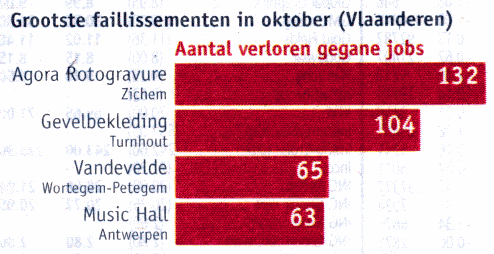
\includegraphics[width=4.5cm]{horizontaal_staafdiagram-faillissementen}
    };
  \end{tikzpicture}
  \begin{enumerate}[(a)]
  \item Welke variabele is er genoteerd bij elke persoon die zijn job is kwijtgeraakt?\\
    \begin{answer}
      Bedrijf waar hij voorheen werkte en de stad waar het bedrijf zich bevond.
    \end{answer}
  \item Welk soort variabele is dat?\\
    \begin{answer}
      Kwalitatief nominaal, met bedrijven of met steden kunnen we niet rekenen.
    \end{answer}
  \item Wat zijn haar waarden?\\
    \begin{answer}
      Agora, gevelbekleding, vandevelde, music hall.
    \end{answer}
  \item Is de figuur goed getekend?\\
    \begin{answer}
      Ja, een staafdiagram moet bestaan uit vrijstaande staafjes waarbij de waarden van de variabelen duidelijk zijn en waarbij ook de frequenties staan. Hier is dit allemaal zo, dat die staafjes horizontaal zijn i.p.v. verticaal is maar opmaak.
    \end{answer}
  \end{enumerate}
\end{frame}

\begin{frame}
  \begin{minipage}{0.45\linewidth}
    \frametitle{Oefening 17}
    Bekijk de tabel over XTC en Speed. Kijk enkel naar de informatie die daarin staat over het jaar 2003.
  \end{minipage}
  \begin{minipage}{0.45\linewidth}
    \vspace*{-1cm}
    \begin{center}
      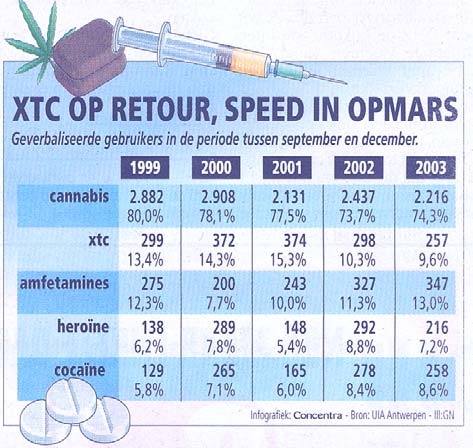
\includegraphics[width=0.8\textwidth]{tabel-drugs}
    \end{center}
  \end{minipage}
  \begin{enumerate}[(a)]
  \item Is “druggebruik” daar behandeld als een kwalitatieve variabele?
    \begin{answer}
      Ja, met kwalitatieve variabelen kunnen we niet rekenen. En met soorten drugs kunnen we niet rekenen. We kunnen het gemiddelde van cannabis en xtc niet bepalen.
    \end{answer}
  \item Is de tabel correct?
    \begin{answer}
      Neen, als we de verschillende relatieve frequenties optellen
      \begin{align*}
        \sum_i{f_i} &= 74.3\%+9.6\%+13.0\%+7.2\%+8.6\%\\[-0.4cm]
                    &= 112.7\%\\
                    &> 100\%
      \end{align*}
      vinden we een getal dat groter is dan het maximum.
    \end{answer}
  \end{enumerate}
\end{frame}

\begin{frame}
  \frametitle{Oefening 18}
  \begin{minipage}{0.35\linewidth}
    Bekijk het taartdiagram over de vrijetijdsbesteding van jongeren.
  \end{minipage}
  \begin{minipage}{0.6\linewidth}
    \vspace*{-1cm}
    \begin{center}
      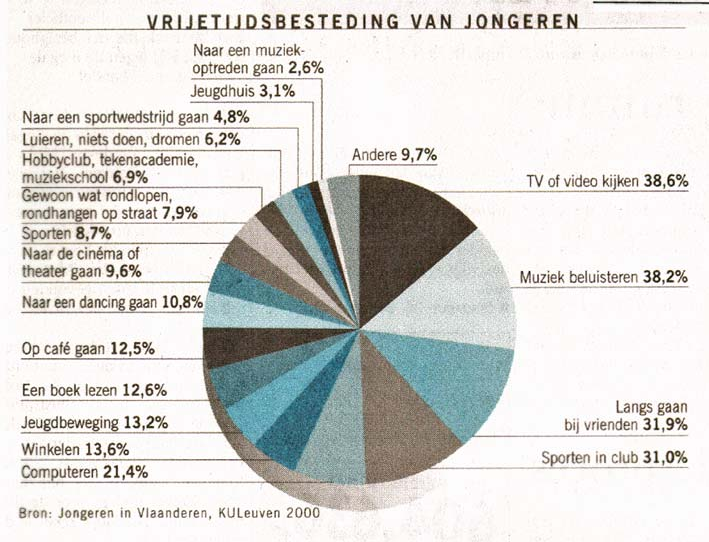
\includegraphics[width=0.8\textwidth]{cirkeldiagram-vrijetijdsbesteding}
    \end{center}
  \end{minipage}
  \begin{enumerate}[(a)]
  \item Is “vrijetijdsbesteding” hier behandeld als een kwalitatieve variabele?\\
    \begin{answer}
      Ja, we kunnen niet rekenen met de variabele. Dus deze moet kwalitatief zijn.
    \end{answer}
  \item Is het taartdiagram correct getekend?\\
    \begin{answer}
      Neen, tel maar eens de eerste paar relatieve frequenties op. Je merkt al snel dat dit niet kan. Hoe is het dan mogelijk dat er überhaupt een diagram kon worden getekend! Dit is de valkuil van automatische tools, deze berekenen eerst de som en gebruiken deze dan om de juiste hoek van een cirkelsector te bepalen.
    \end{answer}
  \end{enumerate}
\end{frame}


\begin{frame}
  \frametitle{Oefening 19}
  Stel een frequentietabel voor de volgende dataset. Kies een verstandige klassenbreedte.
  {\tiny  \dataset[10]{
      193, 225, 256, 166, 143, 260, 117, 208, 182, 114, 113, 203, 320, 231, 221, 231, 60, 113, 373, 180, 379, 205, 161, 287, 196, 236, 163, 192, 184, 166, 332, 172, 227, 272, 264, 155, 296, 189, 119, 230, 253, 225, 194, 200, 91, 177, 208, 157, 243, 183, 89, 235, 190, 223, 186, 132, 235, 312, 125, 258, 98, 173, 165, 289, 262
    }}
  \begin{answer}
    \begin{center}
      \small
      \begin{tabular}{c|c|c|c|c|c}
        $i$ & klasse     & $n_i$ & $cn_i$ & $f_i$ & $cf_i$ \\
        \hline
        1 & $[ 60,  90[$ &   2 & 2 &  0.03 & 0.03\\
        2 & $[ 90, 120[$ &   7 & 9 &  0.11 & 0.14\\
        3 & $[120, 150[$ &   3 & 12 &  0.05 & 0.19\\
        4 & $[150, 180[$ &  10 & 22 & 0.15 & 0.34\\
        5 & $[180, 210[$ &  16 & 38 & 0.25 & 0.59\\
        6 & $[210, 240[$ &  11 & 49 & 0.17 & 0.76\\
        7 & $[240, 270[$ &   7 & 56 & 0.11 & 0.87\\
        8 & $[270, 300[$ &   4 & 60 & 0.06 & 0.93\\
        9 & $[300, 330[$ &   2 & 62 & 0.03 & 0.96\\
        10 & $[330, 360[$ &   1 &63&  0.02 & 0.98\\
        11 & $[360, 390[$ &   2 & 65 & 0.03 & $\approx 1$ \\
      \end{tabular}
    \end{center}
  \end{answer}
\end{frame}

\begin{frame}
  \frametitle{Oefening 20}
  Op de website van de (National Basketball Association) NBA vinden we volgende dataset.
  {\tiny \dataset[10]{
      1.93, 2.22, 2.08, 2.26, 1.98, 2.13, 2.16, 1.94, 1.89, 1.96, 1.92, 2.09, 2.11, 2.09, 2.13, 2, 1.67, 2.08, 2.2, 2.18, 2.18, 2.17, 1.96, 1.95, 2.01, 2.07, 1.74, 1.81, 2.04, 1.99, 1.99, 1.91, 1.74, 2.12, 1.95, 2, 2.25, 2.29, 1.9, 1.98, 2.03, 2.16, 1.82, 2.17, 1.92, 1.99, 1.95, 2, 2, 1.91, 2.26, 2.21, 2.31, 1.91, 2.1, 2.09, 2.17, 1.98, 1.95, 1.96, 2.21, 2.18, 1.96, 1.82, 1.89, 2.21, 2.09, 1.87, 1.83, 2.16, 1.87, 2.18, 2.09, 2.1, 1.7, 2.01, 2.2, 1.67, 1.87, 2.14
    }}
  Maak een goede frequentietabel.
  \begin{answer}
    \begin{center}
      \small
      \begin{tabular}{c|c|c|c|c|c}
        $i$ & klasse        & $n_i$ & $cn_i$ & $f_i$ & $cf_i$ \\
        \hline
        1   & $[ 1.6, 1.7[$ & 2     & 2      & 0.03  & 0.03   \\
        2   & $[ 1.7, 1.8[$ & 3     & 5      & 0.04  & 0.06   \\
        3   & $[ 1.8, 1.9[$ & 9     & 14     & 0.11  & 0.18   \\
        4   & $[ 1.9, 2.0[$ & 22    & 36     & 0.28  & 0.45   \\
        5   & $[ 2.0, 2.1[$ & 16    & 52     & 0.2   & 0.65   \\
        6   & $[ 2.1, 2.2[$ & 17    & 69     & 0.21  & 0.86   \\
        7   & $[ 2.2, 2.3[$ & 10    & 79     & 0.13  & 0.99   \\
        8   & $[ 2.3, 2.4[$ & 1     & 80     & 0.01  & 1      \\
      \end{tabular}
    \end{center}
  \end{answer}
  {\tiny Door afrondingsfouten kunnen er in bovenstaande oplossing kleine verschillen zitten.}
\end{frame}

\begin{frame}
  \frametitle{Oefening 21}
  In een klas met 24 leerlingen geef ik een onverwachte toets op 10. Volgende resultaten werden behaald en op score geplaatst:
  \begin{center}
    \tiny
    \dataset[8]{
      7.5, 9, 9, 5.5, 8.5, 7.5, 7, 9, 7.5, 3, 8.5, 6, 8, 8.5, 7.5, 8, 9, 7, 9, 7, 7, 8, 6, 8
    }
  \end{center}
  Is het hier nodig om een frequentietabel te maken met klassen?
  \begin{answer}
    Het kan m.b.v. een frequentietabel, punten kunnen we zien als een kwantitatieve discrete dataset. Alternatief kunnen we dit ook opvatten als een kwalitatief ordinale dataset, waarbij punten zoals 3 slecht zijn en punten zoals 8 en 9 zeer goed zijn.
  \end{answer}
\end{frame}

\begin{frame}
  \frametitle{Oefening 22}
  \begin{minipage}{0.60\linewidth}
    Teken het histogram en het frequentiepolygoon horende bij volgende frequentietabel.\\
  \end{minipage}
  \begin{minipage}{0.35\linewidth}
    \begin{center}
      \tiny
      \begin{tabular}{c|c|c|c}
        $i$ & klasse     & $n_i$ & $f_i$\\
        \hline
        1 & $[ 60,  90[$ &   2 &  0.03\\
        2 & $[ 90, 120[$ &   7 &  0.11\\
        3 & $[120, 150[$ &   3 &  0.05\\
        4 & $[150, 180[$ &  10 &  0.15\\
        5 & $[180, 210[$ &  16 &  0.25\\
        6 & $[210, 240[$ &  11 &  0.17\\
        7 & $[240, 270[$ &   7 &  0.11\\
        8 & $[270, 300[$ &   4 &  0.06\\
        9 & $[300, 330[$ &   2 &  0.03\\
        10 & $[330, 360[$ &   1 &  0.02\\
        11 & $[360, 390[$ &   2 &  0.03\\
      \end{tabular}
    \end{center}
  \end{minipage}
  \begin{answer}
    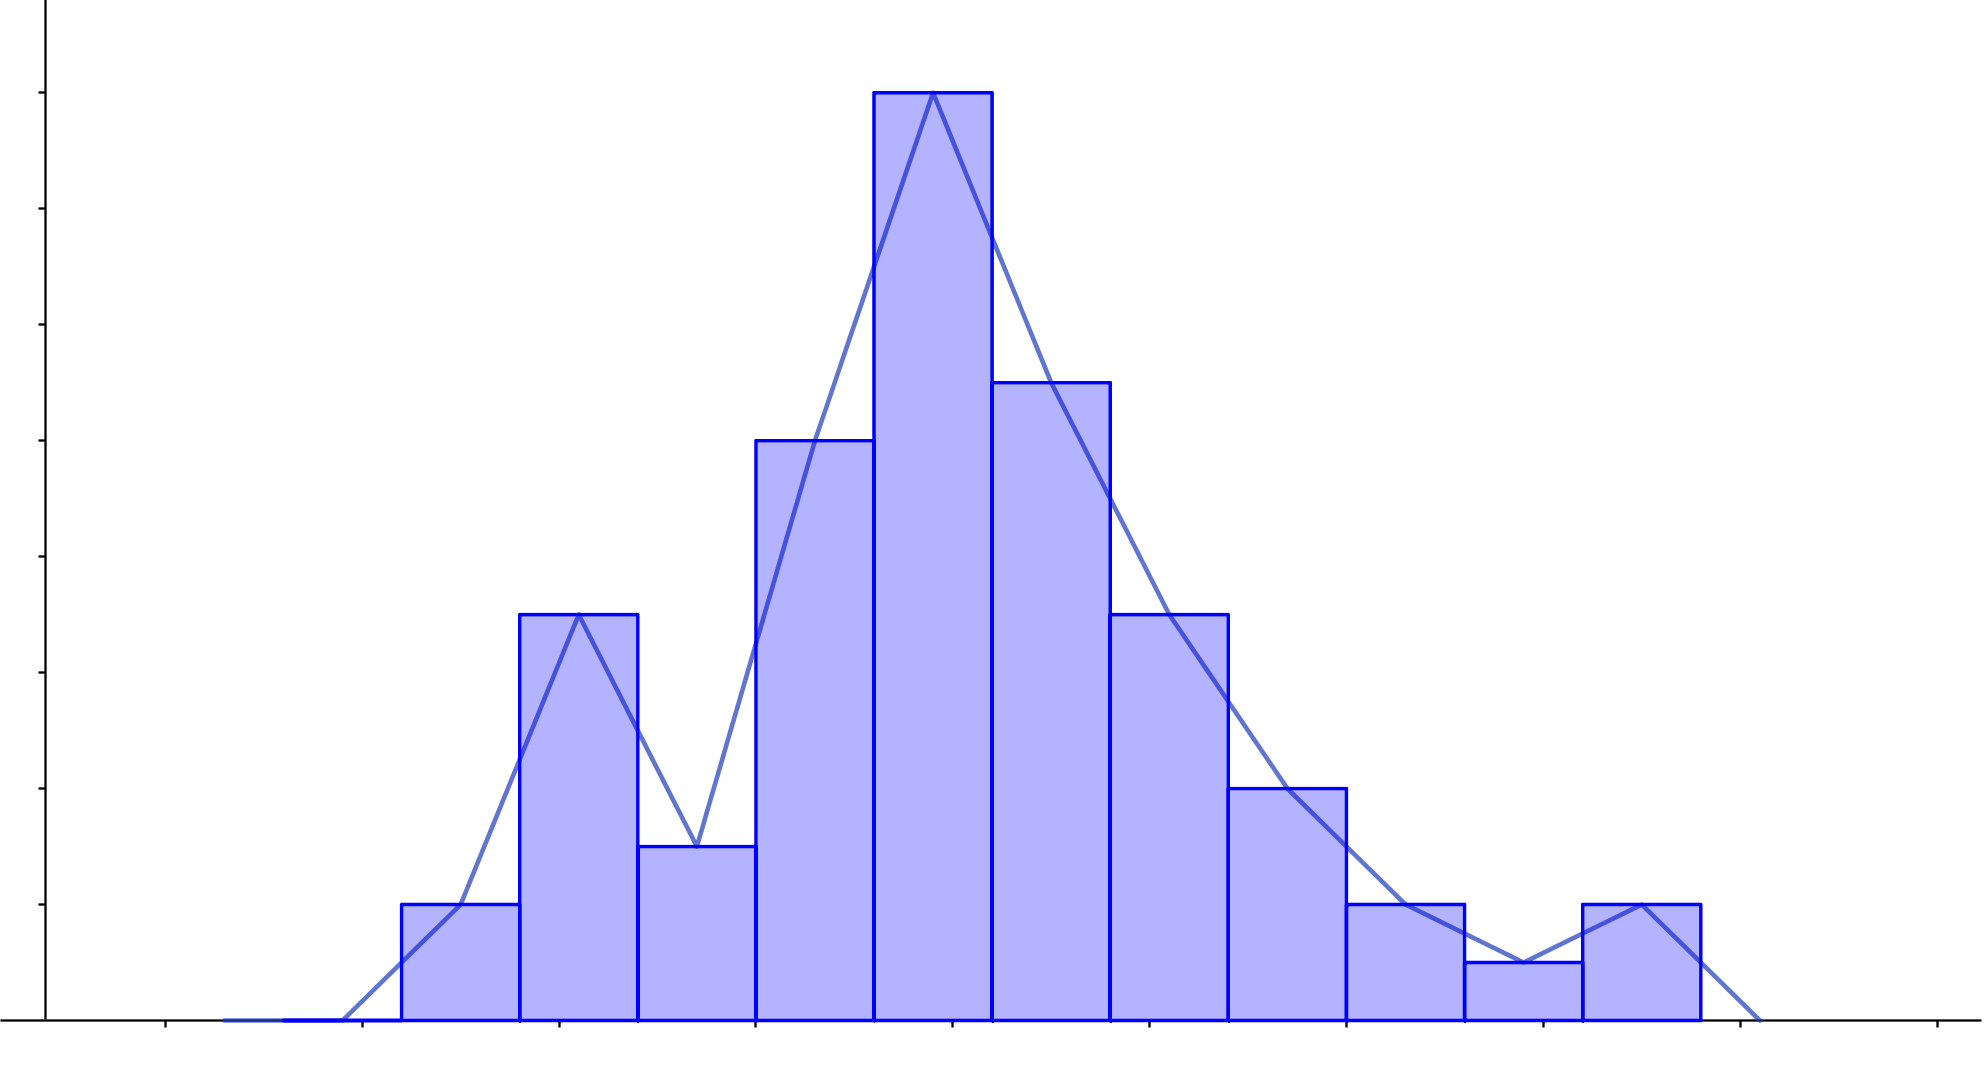
\includegraphics[width=\linewidth]{WachttijdenLesHistogram}
  \end{answer}
\end{frame}

\begin{frame}
  \frametitle{Oefening 23}
  In een klas met 24 leerlingen geef ik een onverwachte toets op 10. Volgende resultaten werden behaald en op score geplaatst:
  \begin{center}
    {\tiny \dataset[8] {
        7.5, 9, 9, 5.5, 8.5, 7.5, 7, 9, 7.5, 3, 8.5, 6, 8, 8.5, 7.5, 8, 9, 7, 9, 7, 7, 8, 6, 8
      }}
  \end{center}
  \begin{minipage}{.6\linewidth}
    \begin{enumerate}[(a)]
    \item Maak een frequentietabel met zowel de waarnemingen als de klassen gelijke frequentie.\\
      \begin{answer}
        Zie hiernaast.
      \end{answer}
    \item Maak dan een staafdiagram.\\
      \begin{answer}
        Gebruik de waarnemingen, hou rekening met de plaats tussen de staafjes en de orde.
      \end{answer}
    \item Maak dan een histogram.\\
      \begin{answer}
        Gebruik nu de klassen.
      \end{answer}
    \end{enumerate}
  \end{minipage}
  \begin{minipage}{0.35\linewidth}
    \begin{answer}
    \begin{center}
      \small
      \begin{tabular}{c|c|c}
        waarneming & klasse    & $n_i$ \\
        \hline
        $3$        & $[3,3.5[$ & 1     \\
        $3.5$      & $[3.5,4[$ & 0     \\
        $4$        & $[4,4.5[$ & 0     \\
        $4.5$      & $[4.5,5[$ & 0     \\
        $5$        & $[5,5.5[$ & 0     \\
        $5.5$      & $[5.5,6[$ & 1     \\
        $6$        & $[6,6.5[$ & 2     \\
        $6.5$      & $[6.5,7[$ & 0     \\
        $7$        & $[7,7.5[$ & 4     \\
        $7.5$      & $[7.5,8[$ & 4     \\
        $8$        & $[8,8.5[$ & 4     \\
        $8.5$      & $[8.5,9[$ & 3     \\
        $9$        & $[9,9.5[$ & 5     \\
      \end{tabular}
    \end{center}
  \end{answer}
  \end{minipage}
\end{frame}

\begin{frame}
  \frametitle{Oefening 24}
  \begin{minipage}{0.5\linewidth}
  Als je de groottes van de basketbalspelers in acht klassen hebt opgedeeld krijgen we volgende frequentietabel. Maak zelf het bijhorende histogram en teken het frequentiepolygoon.\\
\end{minipage}
\begin{minipage}{0.4\linewidth}
  \begin{center}
    \begin{tabular}{c|c|c}
      $i$ & klasse     & $n_i$\\
      \hline
      1 & $[ 1.60,  1.70[$ &   2\\
      2 & $[ 1.70,  1.80[$ &   3\\
      3 & $[ 1.80,  1.90[$ &   9\\
      4 & $[ 1.90,  2.00[$ &   22\\
      5 & $[ 2.00,  2.10[$ &   16\\
      6 & $[ 2.10,  2.20[$ &   17\\
      7 & $[ 2.20,  2.30[$ &   10\\
      8 & $[ 2.30,  2.40[$ &   1\\
    \end{tabular}
  \end{center}
\end{minipage}
\vspace*{-1cm}
\begin{center}
  \begin{answer}
    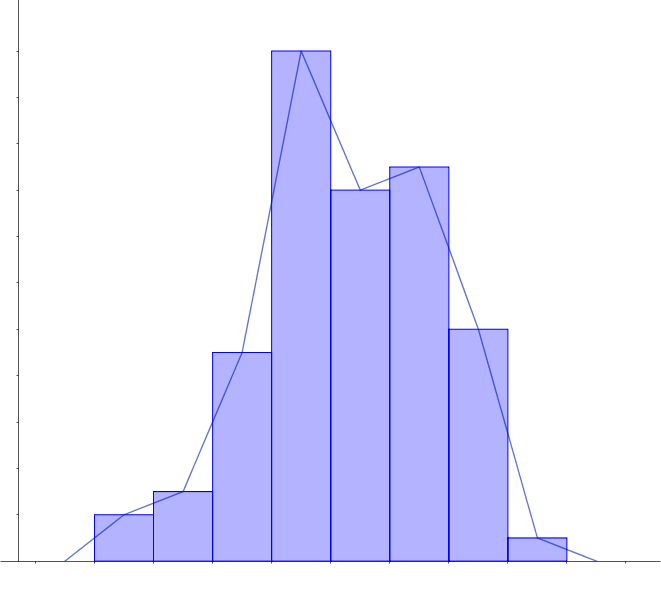
\includegraphics[width=0.5\linewidth]{GrootteBasketbalSpelersHistogram}
  \end{answer}
\end{center}
\end{frame}

\end{document}

